\lesson{Quantum Theory}
The energy of a photon of electromagnetic radiation is \textbf{proportional} to its frequency,
not to its intensity/brightness as had been believed up to that time. This is used to derive
the Planck equation
\[
    E=h\nu
\]
Where $E$ is the energy, $h=6.63\times10^{-34}\,\si{J.s}$, the Planck constant, and $\nu=$ the
frequency of the wave.\\

\subsection{Flaw with Rutherford's Model}
\begin{bulleted-list}
    \item Rutherford believed that the electrons orbited around the nucleus like planets
    \item Only problem was that they should be emitting energy, meaning that they would eventually
        collapse into the nucleus. See Figure \ref{fig:rutherford-model-flaw}
    \item This would leave the atom unstable, so chemists knew this was not the case
\end{bulleted-list}

\begin{figure}[ht!]
    \centering
    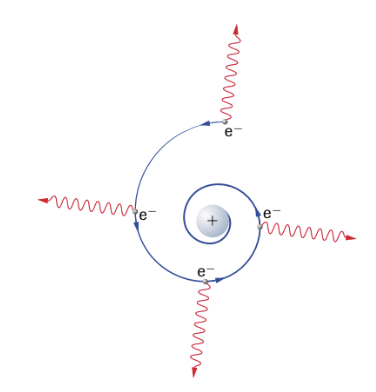
\includegraphics[width=0.4 \textwidth]{../figures/rutherford-model-flaw.png}
    \caption{According to Rutherford's model, an obiting electron should continuously emit
            electromagnetic radiation, losing energy, and collapse the atom. The evidence is to the
            contrary}
    \label{fig:rutherford-model-flaw}
\end{figure}

\subsection{Atomic Spectra}
\begin{bulleted-list}
    \item Robert Bunsen and Gustav Kirchhoff worked together to invent the \textbf{spectroscope}.
        See Figure \ref{fig:spectroscope}
    \item The spectroscope forms the basis of an analytic method called \textbf{spectroscopy}
        \footnote{
            \textbf{Spectroscopy:} a tehcnique for analyzing spectra; the spectra may be visible
            light, infrared, ultraviolet, X-ray, and other types
        }
    \item Bunsen and Kirchhoff studied the spectra of chemicals, especially elements, heated in
        a Bunsen burner flame, and the spectrum of the Sun. They discovered that an element not
        only produced a characteristic flame colour but, on closer examination through a
        spectroscope, also produced a \textbf{bright-line spectrum}
        \footnote{
            \textbf{Bright-line spectrum:} a series of bright lines of light produced or emitted by
            a gas excited by, for example, heat or electricity
        }
        that was characteristic of
        the element
    \item This techique was used to catalogue known elements and when a new spectrum was found,
        the spectrum was used as evidence of a new element
    \item The elements \textbf{cesium} and \textbf{rubidium} were discovered within a year of
        the invention of spectroscopy
    \item \textbf{Note:} spectroscopes may separate the light by using a prism, or a
        \textbf{diffraction grating}. The most modern, compact, and inexpensive school spectrometers
        use a diffraction grating
\end{bulleted-list}

\begin{important}
    Different elements have different spectrums because they have different number of protons,
    and different arrangement of electrons. The differences in spectra reflects the differences
    in the amount of energy that the atoms absorb or give off when their electrons move between
    energy levels. Hence, this is an effective technique in identifying new elements.
\end{important}

\begin{figure}[ht!]
    \centering
    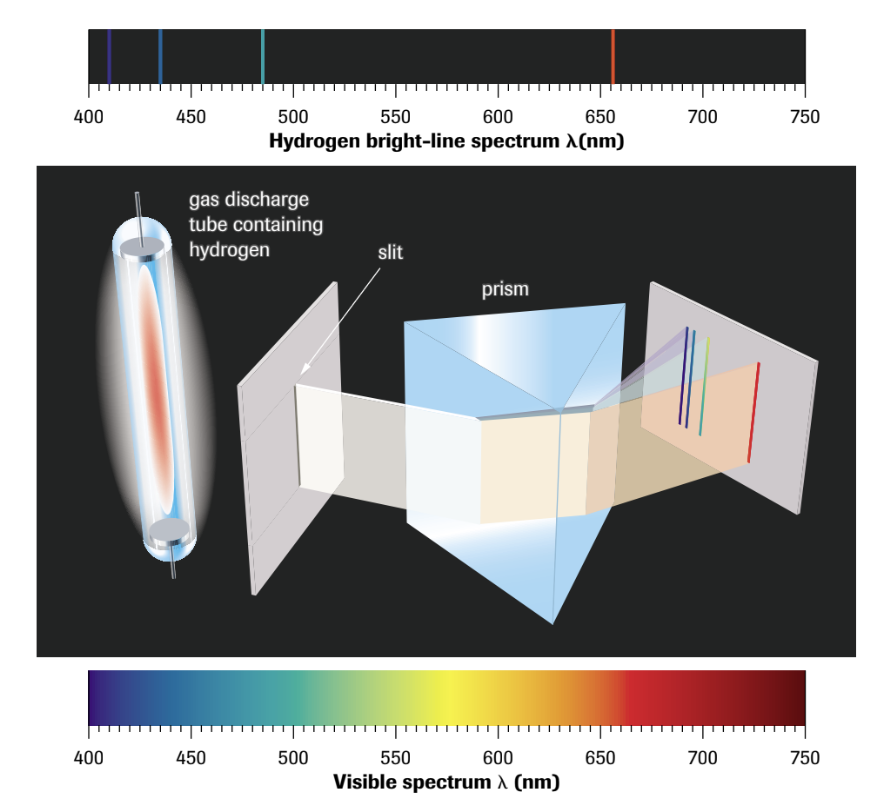
\includegraphics[width=0.9 \textwidth]{../figures/spectroscope.png}
    \caption{Light from a source of light is passed through slits to form a narrow beam. This beam
            is split into its components by the prism to produce a series of coloured lines. The visible region
            of the hydrogen spectrum includes four coloured lines at the wavelengths shown by the scale}
    \label{fig:spectroscope}
\end{figure}

\begin{bulleted-list}
    \item Around 1814, \textbf{absorption} or \textbf{dark-line spectra} were investigated by
        Joseph von Fraunhofer
    \item Kirchhoff, among others, was able to show in the 1860s that dark lines in an element's
        spectrum were in the same position as the bright lines in the spectrum of the same element.
        See Figure \ref{fig:dark-line-spectrum}
    \item This provided a powerful tool to determine the composition of gases far away in the
        universe. When light passes through a gas, for example, the atmosphere around the Sun,
        some light is absorbed by the atoms present in the gas
\end{bulleted-list}

\begin{figure}[ht!]
    \centering
    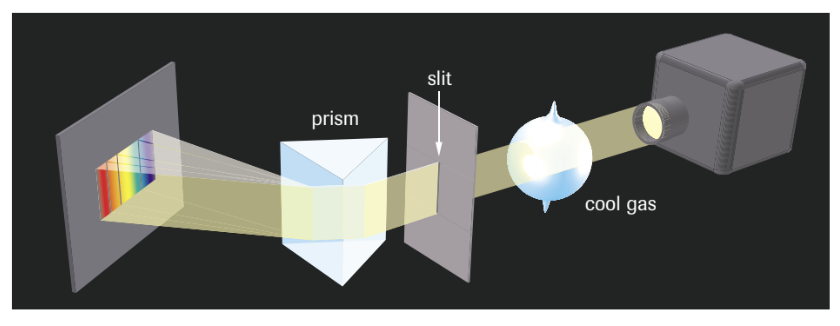
\includegraphics[width=0.9 \textwidth]{../figures/dark-line-spectrum.png}
    \caption{If you start with a complete colour spectrum of all possible colours, then pass this
            light through a gas and analyze what is left, you get a dark-line spectrum; in other words,
            the complete spectrum with some lines missing.}
    \label{fig:dark-line-spectrum}
\end{figure}

\subsection{Bohr's Model}
\begin{definition}{Bohr's First Postulate}
    Electrons do not radiate energy as they orbit the nucleus. Each orbit corresponds to a state
    of constant energy called a \textbf{stationary state}.
\end{definition}

\begin{bulleted-list}
    \item Bohr reasoned that if the light released or absorbed from an atom was quantized, then the
        energy of the electron inside the atom must also be quantized. In other words, an electron
        can only have certain energies. The simplest arrangement would be a planetary model with
        each electron orbit at a fixed distance with a fixed energy
    \item Electrons do move in a circular orbit around the nucleus, with the motion described
        by classical physics
    \item Electrons have only a \textbf{fixed set of allowed orbits}, called \textbf{stationary states}.
        \footnote{
            \textbf{Stationary state:} a stable energy state of an atomic system that does not
            involve any emission of radiation.
        }
        Stationary in the sense that the energy is constant.
        As long as an electron remains in its orbit, its energy is constant and gives off no energy
    \item An electron can only pass from one allowed orbit to another. That is, electrons cannot
        lie between orbits
\end{bulleted-list}

\begin{definition}{Bohr's Second Postulate}
    Electrons can change their energy only by undergoing a \textbf{transition} from one stationary 
    state to another.
\end{definition}

\begin{bulleted-list}
    \item Bohr observed the spectrum lines when observing hydrogen. The non-continuous
        colours suggested only certain energies were released. See Figure \ref{fig:hydrogen-spectrum-lines}
    \item There are two states for electrons:
        \begin{enum}
            \item \textbf{Ground state:} the ``expected'' arrangement of electrons. This is because
                this is the lowest amount of energy the electrons can possess
            \item \textbf{Excited state:} When an electron temporarily occupies an energy state higher
                than its ground state--it transitioning between energy levels. The more energy the 
                electron absorbed, the higher the energy levels the electrons can move to. 
                Eventually, the electron returns back to the ground state, releasing energy
                in the form of \textbf{photons}. This is called an electron \textbf{transition}.
                \footnote{
                    \textbf{Transition:} the jump of an electron from one stationary state to
                    another.
                }
        \end{enum}
    \item A transition from a higher energy state to a lower energy state means that the electron
        loses energy and this energy is released as a photon of light, explaining a bright line
        in a bright-line spectrum. When some energy is absorbed, for example from a photon of
        light, the electron undergoes a transition from a lower energy state to a higher one,
        explaining a dark line in an absorption spectrum. These dark lines indicate the amount
        of energy that was absorbed when the electrons transitioned. See Figure \ref{fig:bohr-model-electron-transition}
\end{bulleted-list}

\begin{figure}[ht!]
    \centering
    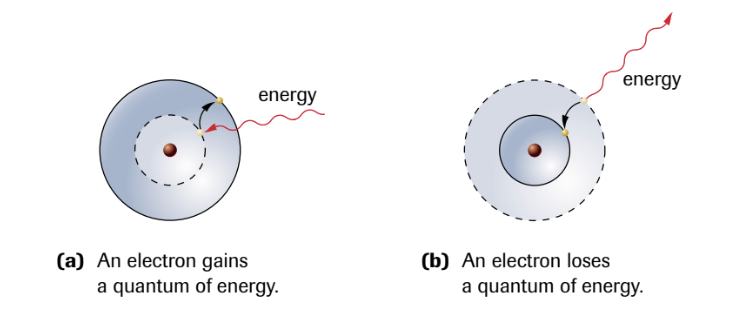
\includegraphics[width=0.4 \textwidth]{../figures/bohr-model-electron-transition.png}
    \caption{}
    \label{fig:bohr-model-electron-transition}
\end{figure}

\begin{figure}[ht!]
    \centering
    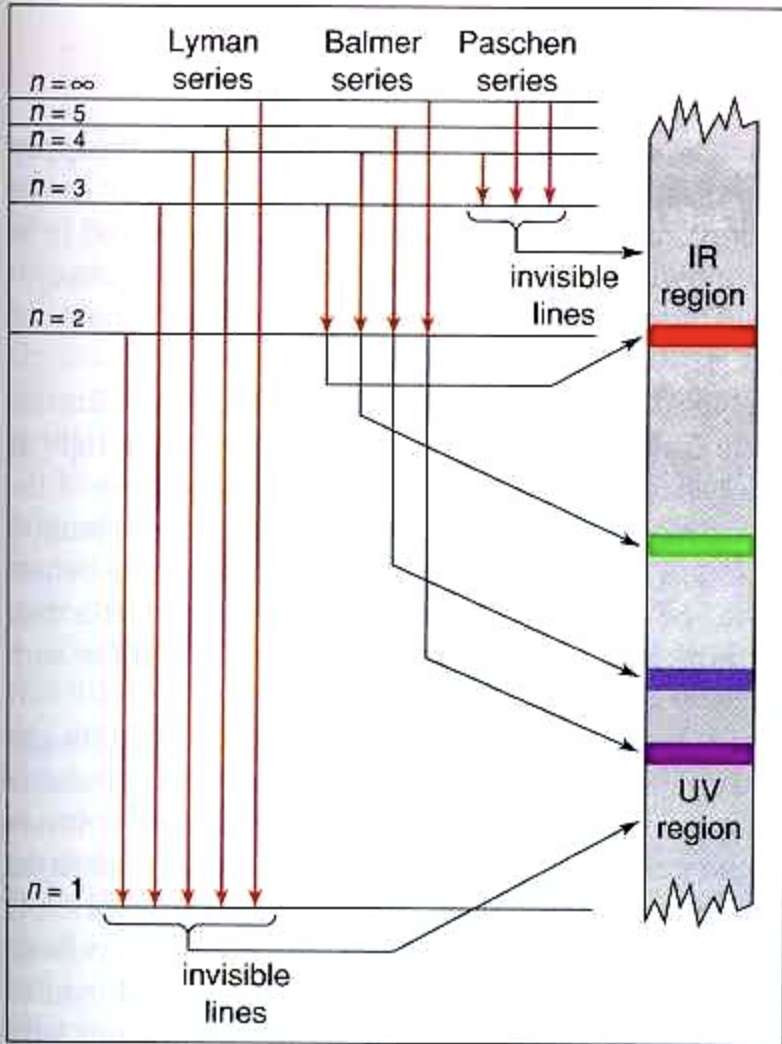
\includegraphics[width=0.4 \textwidth]{../figures/hydrogen-spectrum-lines.png}
    \caption{Because there are so many atoms, and thus a lot of electrons, in a sample of hydrogen 
            gas, there would be a continuous spectrum and not individual lines. These lines indicate
            that energy is released in quanta and not continuous}
    \label{fig:hydrogen-spectrum-lines}
\end{figure}

\subsection{The Successes and Failures of the Bohr Model}
\textbf{Successes}
\begin{bulleted-list}
    \item The Bohr model of the atom is able to offer a reasonable explanation of Mendeleev's
        periodic law and its representation in the periodic table
    \item According to the Bohr model, periods in the periodic table result from the filling of
        electron energy levels in the atom. E.g., atoms in Period 3 have electrons in 3 energy
        levels
    \item Although Bohr did his calculations as if electrons were in circular orbits, the most
        important property of the electrons was their energy, not their motion
    \item Bohr's model was also able to successfully predict the infrared and ultra-violet spectra
        for hydrogen
\end{bulleted-list}
\textbf{Failures}
\begin{bulleted-list}
    \item It only works very well for the spectrum of hydrogen atoms, or ions with only one
        electron
    \item The calculations of spectral lines using Bohr's theory for any atom or ion containing
        more than one electron did not agree with the empirical results
    \item The disrepancy became worse as the number of electrons increased
        \footnote{
            Despite the failures, Bohr's theory was a great success because it was the start
            of a new approach--including the new quantum ideas in a model of the atom
        }
\end{bulleted-list}

\begin{sample}{Use the Bohr theory and the periodic table to draw energy-level diagrams for
    the phosphrous atom.}
    Phosphorus is in period 3--there are 2, 8, and 5 electrons per energy level. To draw
    the energy-level diagram, work from the bottom up:
    \begin{table}[!ht]
        \centering
        \setlength{\tabcolsep}{12pt}      % column spacing
        \renewcommand{\arraystretch}{1.2} % row spacing
        \arrayrulecolor{black}            % table border color
        \begin{tabularx}{\textwidth}{
                >{\hsize=0.4\hsize}X
                >{\hsize=0.1\hsize}X
                >{\hsize=0.5\hsize}X
            }
            Sixth, the 3rd energy level, & 5 \si{e^-} & (from group \textbf{15})\\
            Fifth, the 2nd energy level, & 8 \si{e^-} & (from eight elements in \textbf{period 2})\\
            Fourth, the 1st energy level & 2 \si{e^-} & (from two elements in \textbf{period 1})\\
            Third, the protons: & 15 \si{p^+} & (from the \textbf{atomic number})\\
            Second, the symbol: & P & (uppercase symbol from the table)\\
            First, the name of the atom & phosphorus & (lowercase name)
        \end{tabularx}
    \end{table}
\end{sample}

\begin{sample}{Use the Bohr theory and the periodic table to draw energy-level diagrams for
    hydrogen, carbon, and sulfur atoms.}
    Using the same method as above
    \begin{table}[!ht]
        \centering
        \setlength{\tabcolsep}{12pt}      % column spacing
        \renewcommand{\arraystretch}{1.2} % row spacing
        \arrayrulecolor{black}            % table border color
        \begin{tabularx}{\textwidth}{X X X}
             & & 6 \si{e^-} \\
             & 4 \si{e^-} & 8 \si{e^-} \\
            1 \si{e^-} & 2 & 2 \si{e^-} \\
            1 \si{p^+} & 6 \si{p^+} & 16 \si{p^+} \\
            H & C & S \\
            hydrogen & carbon & sulfur
        \end{tabularx}
    \end{table}
\end{sample}

\begin{tabularx-custom}{|X X|}{Creating the Bohr Atomic Theory (1913)}
    Key experimental evidence & Theoretical explanation \\
    Mendeleev (1869-1872): there is a periodicity of the physical and chemical properties
    of the elements & A new period begins in the periodic table when a new energy level of electrons
    is started in the atom \\ \hline
    Mendeleev (1872): there are two elements in the first period and eight elements in the second
    period of the periodic table & There are two electrons in the first energy level and eight
    in the next level \\ \hline
    Kirchhoff, Bunsen (1859), Johann Balmer (1885): emission and absorption of line spectra, and
    not continuous spectra, exist for gaseous elements & Since the energy of light absorbed and
    emitted is quantized, the energy of electrons in atoms is quantized \\ \hline
\end{tabularx-custom}

\subsection{Timeline}
Figure \ref{fig:timeline} is the timeline up to the Bohr model.

\begin{figure}[ht!]
    \centering
    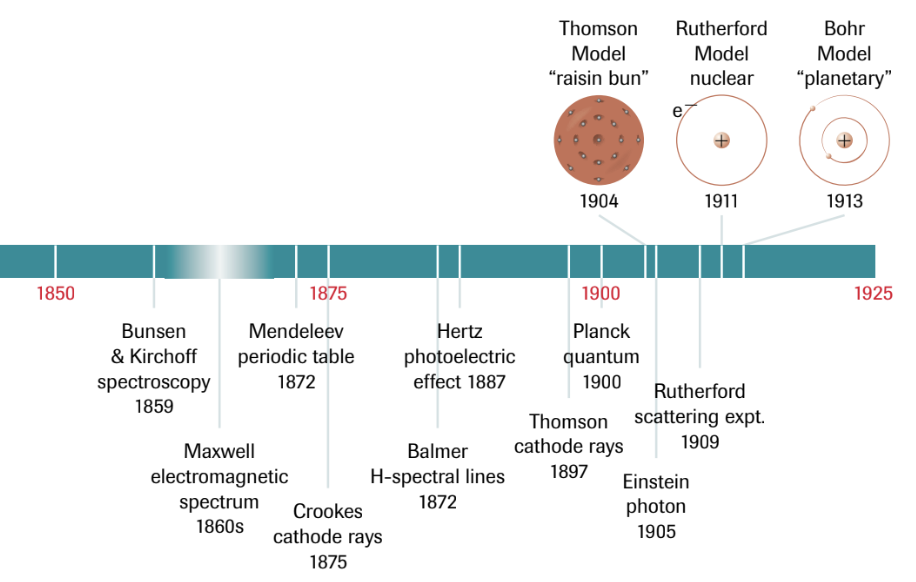
\includegraphics[width=0.8 \textwidth]{../figures/timeline.png}
    \caption{In a little over a hundred years, the idea of an atom has changed from the original
            indivisible sphere of Dalton to a particle with several components and an internal
            organization}
    \label{fig:timeline}
\end{figure}

\begin{problems}
    \item What was the main achievement of the Rutherford model? What was the main problem with
        this model?
    \item State Bohr's solution to the problem with the Rutherford atomic model.
    \item When creating his new atomic theory, Bohr used one important new idea (theory) and
        primarily one important experimental area of study. Identify each of these.
    \item 
        \begin{enum-alph}
            \item What is the empirical distinction between emission and absorption spectra?
            \item In general terms, how did Niels Bohr explain each one of these spectra?
        \end{enum-alph}
    \item Draw an energy-level diagram for each of the following:
        \begin{enum-alph}
            \item Fluorine atom
            \item Neon atom
            \item Sodium atom
        \end{enum-alph}
    \item What do the atomic, periodic, and group numbers contribute in energy-level diagrams?
    \item State two or more reasons why Bohr's theory was considered a success.
    \item Identify one significant problem with the Bohr theory.
    \item In 1885, Balmer created an equation that described the visible light spectrum for
        hydrogen. This evolved to become the Rydberg equation presented below. Bohr used Balmer's
        work as an insight into the structure of the hydrogen atom.
        \[
            \frac{1}{\lambda}=R_H\left(\frac{1}{n_f^2}-\frac{1}{n_i^2}\right)
        \]
        Where $R_H=1.10\times10^7\,\si{m^{-1}}$.
        \footnote {
            The alternative Ryderberg equation, $\Delta E=-R_H\left(\frac{1}{n_f^2}-\frac{1}{n_i^2}\right)$,
            where $R_H=2.18\times10^{-18}\,\si{J}$, is derived by using the equation $\Delta E=\frac{hc}{\lambda}$
        }
        \begin{enum-alph}
            \item The visible portion of the hydrogen spectrum is called the Balmer series. The
                visible light photons emitted from the hydrogen atom all involve electron
                transitions from higher (excited) energy levels down to the $n_f=2$ level. Calculate
                the wavelength of the light emitted from the quantum leap of an electron from
                $n_i=4$ to $n_f=2$.
            \item Use the wave equation, $\lambda=\frac{c}{\nu}$, to calculate the frequency of
                the light emitted.
            \item Use the Planck equation, $E=h\nu$, to calculate the energy of the electron
                transition and, therefore, the difference in energy between the $n_i=4$ and the $n_f=2$
                levels
            \item Repeat (a) through (c) for the $n_i=3$ to the $n_f=2$ electron transition.
            \item Draw an energy-level diagram for hydrogen showing the $n_i=3$ and 4
                to the $n_f=2$ transitions. Add the energy difference values to the diagram.
                From these values, what is the energy difference between $n=4$ and $n=3$?
        \end{enum-alph}
    \item Using your knowledge of the history of atomic theories from Dalton to Bohr, state what
        you think will happen next in the historical story.
\end{problems}
\begin{solutions}
    \item The main achievement of the Rutherford model was the discovery of the nucleus. This
        model proposed that electrons orbited the nucleus in a solar system like fashion. The
        problem with this model is that the electrons emit electromagnetic radiation when orbiting,
        meaning that they would eventually collapse into the nucleus
    \item Bohr's solution was that these electrons orbited in stationary states around the nucleus.
        Each electron orbited the nucleus in a fixed energy level and maintained a constant
        energy when orbiting. This way, the electrons do not lose energy and collapse into
        the nucleus.
    \item 
        \begin{enum-alph}
            \item Emission spectra consist of light emitted by a sample of substance. Absorptions
                spectra consist of missing frequencies (colours) of light after the source light
                passes through a sample of substance.
            \item Bohr explained each one of these spectra as energy being emitted by electrons 
                transitioning from a higher energy state to a lower energy state, emitting
                energy in the form of protons
        \end{enum-alph}
    \item 
        \begin{enum-alph}
            \item Fluorine has 9 protons and electrons
                \begin{align*}
                    &7\,\si{e^-}\\
                    &2\,\si{e^-}\\
                    &9\,\si{p^+}\\
                    &\text{F}
                    &\text{fluorine}
                \end{align*}
            \item Neon has 10 protons and electrons
                \begin{align*}
                    &8\,\si{e^-}\\
                    &2\,\si{e^-}\\
                    &10\,\si{p^+}\\
                    &\text{Ne}
                    &\text{neon}
                \end{align*}
            \item Sodium has 11 protons and electrons
                \begin{align*}
                    &1\,\si{e^-}\\
                    &8\,\si{e^-}\\
                    &2\,\si{e^-}\\
                    &11\,\si{p^+}\\
                    &\text{Na}
                    &\text{sodium}
                \end{align*}
        \end{enum-alph}
    \item The atomic number is the number of protons and electrons the atom has, the period
        is the number of energy levels the atom has, and the group number is the number of
        valence electrons the atom has.
    \item Bohr's theory explained the known emission spectral lines for hydrogen, the periodic trend 
        in Mendeleev's periodic table, helped predict UV and infrared spectra for hydrogen, and solved 
        the problem with the Rutherford model.
    \item The Bohr theory only worked well for the spectrum of hydrogen atoms, or ions with only
        one electron. Calculations for spectrum lines with this theory didn't match with empircal
        evidence. The disrepancy became worse as the number of electrons increased.
    \item 
        \begin{enum-alph}
            \item Using the equation
                \begin{align*}
                    \frac{1}{\lambda}&=(1.10\times10^7\,\si{m^{-1}})\left(\frac{1}{2^4}-\frac{1}{4^2}\right)\\
                    \frac{1}{\lambda}&=(1.10\times10^7\,\si{m^{-1}})\left(\frac{3}{16}\right)\\
                    \lambda&=\frac{16}{3.30\times10^7\,\si{m^{-1}}}\\
                           &=4.85\times10^{-7}\,\si{m}
                \end{align*}
            \item Substituting into the equation
                \begin{align*}
                    \nu&=\frac{c}{\lambda}\\
                       &=\frac{3.0\times10^8\,\si{m.s^{-1}}}{4.85\times10^{-7}\,\si{m}}\\
                       &=6.19\times10^{14}\,\si{Hz}
                \end{align*}
            \item Substituting into the equation
                \begin{align*}
                    E&=(6.63\times10^{-34}\,\si{J.s})(6.19\times10^{14}\,\si{Hz})\\
                     &=4.10\times10^{-19}\,\si{J}
                \end{align*}
                However, because the electron is moving from the $n_i=4$ to $n_f=2$ level, energy is released,
                meaning that the sign of our final answer should be negative. Thus
                \[
                    E=-4.10\times10^{-19}\,\si{J}
                \]
            \item We will skip the steps and use the alternative Rydberg equation
                \begin{align*}
                    \Delta E&=-R_H\left(\frac{1}{n_f^2}-\frac{1}{n_i^2}\right)\\
                            &=-(2.18\times10^{-18}\,\si{J})\left(\frac{1}{2^2}-\frac{1}{3^2}\right)\\
                            &=-3.03\times10^{-19}\,\si{J}
                \end{align*}
            \item This is the same diagram seen in Figure \ref{fig:hydrogen-spectrum-lines}. The difference
                in energy is $4.10\times10^{-19}\,\si{J}-3.03\times10^{-19}\,\si{J}=1.07\times10^{-19}\,\si{J}$.
        \end{enum-alph}
    \item The most likely assumption is that theories would advance to try and describe arrangements
        and energies for atoms more complex than hydrogen.
\end{solutions}
